    % Appendix A

\chapter{Diagrama de \textit{User Flow}} % Main appendix title

\label{app:userflowchart}

\begin{figure}[h!tbp]
    \centering
    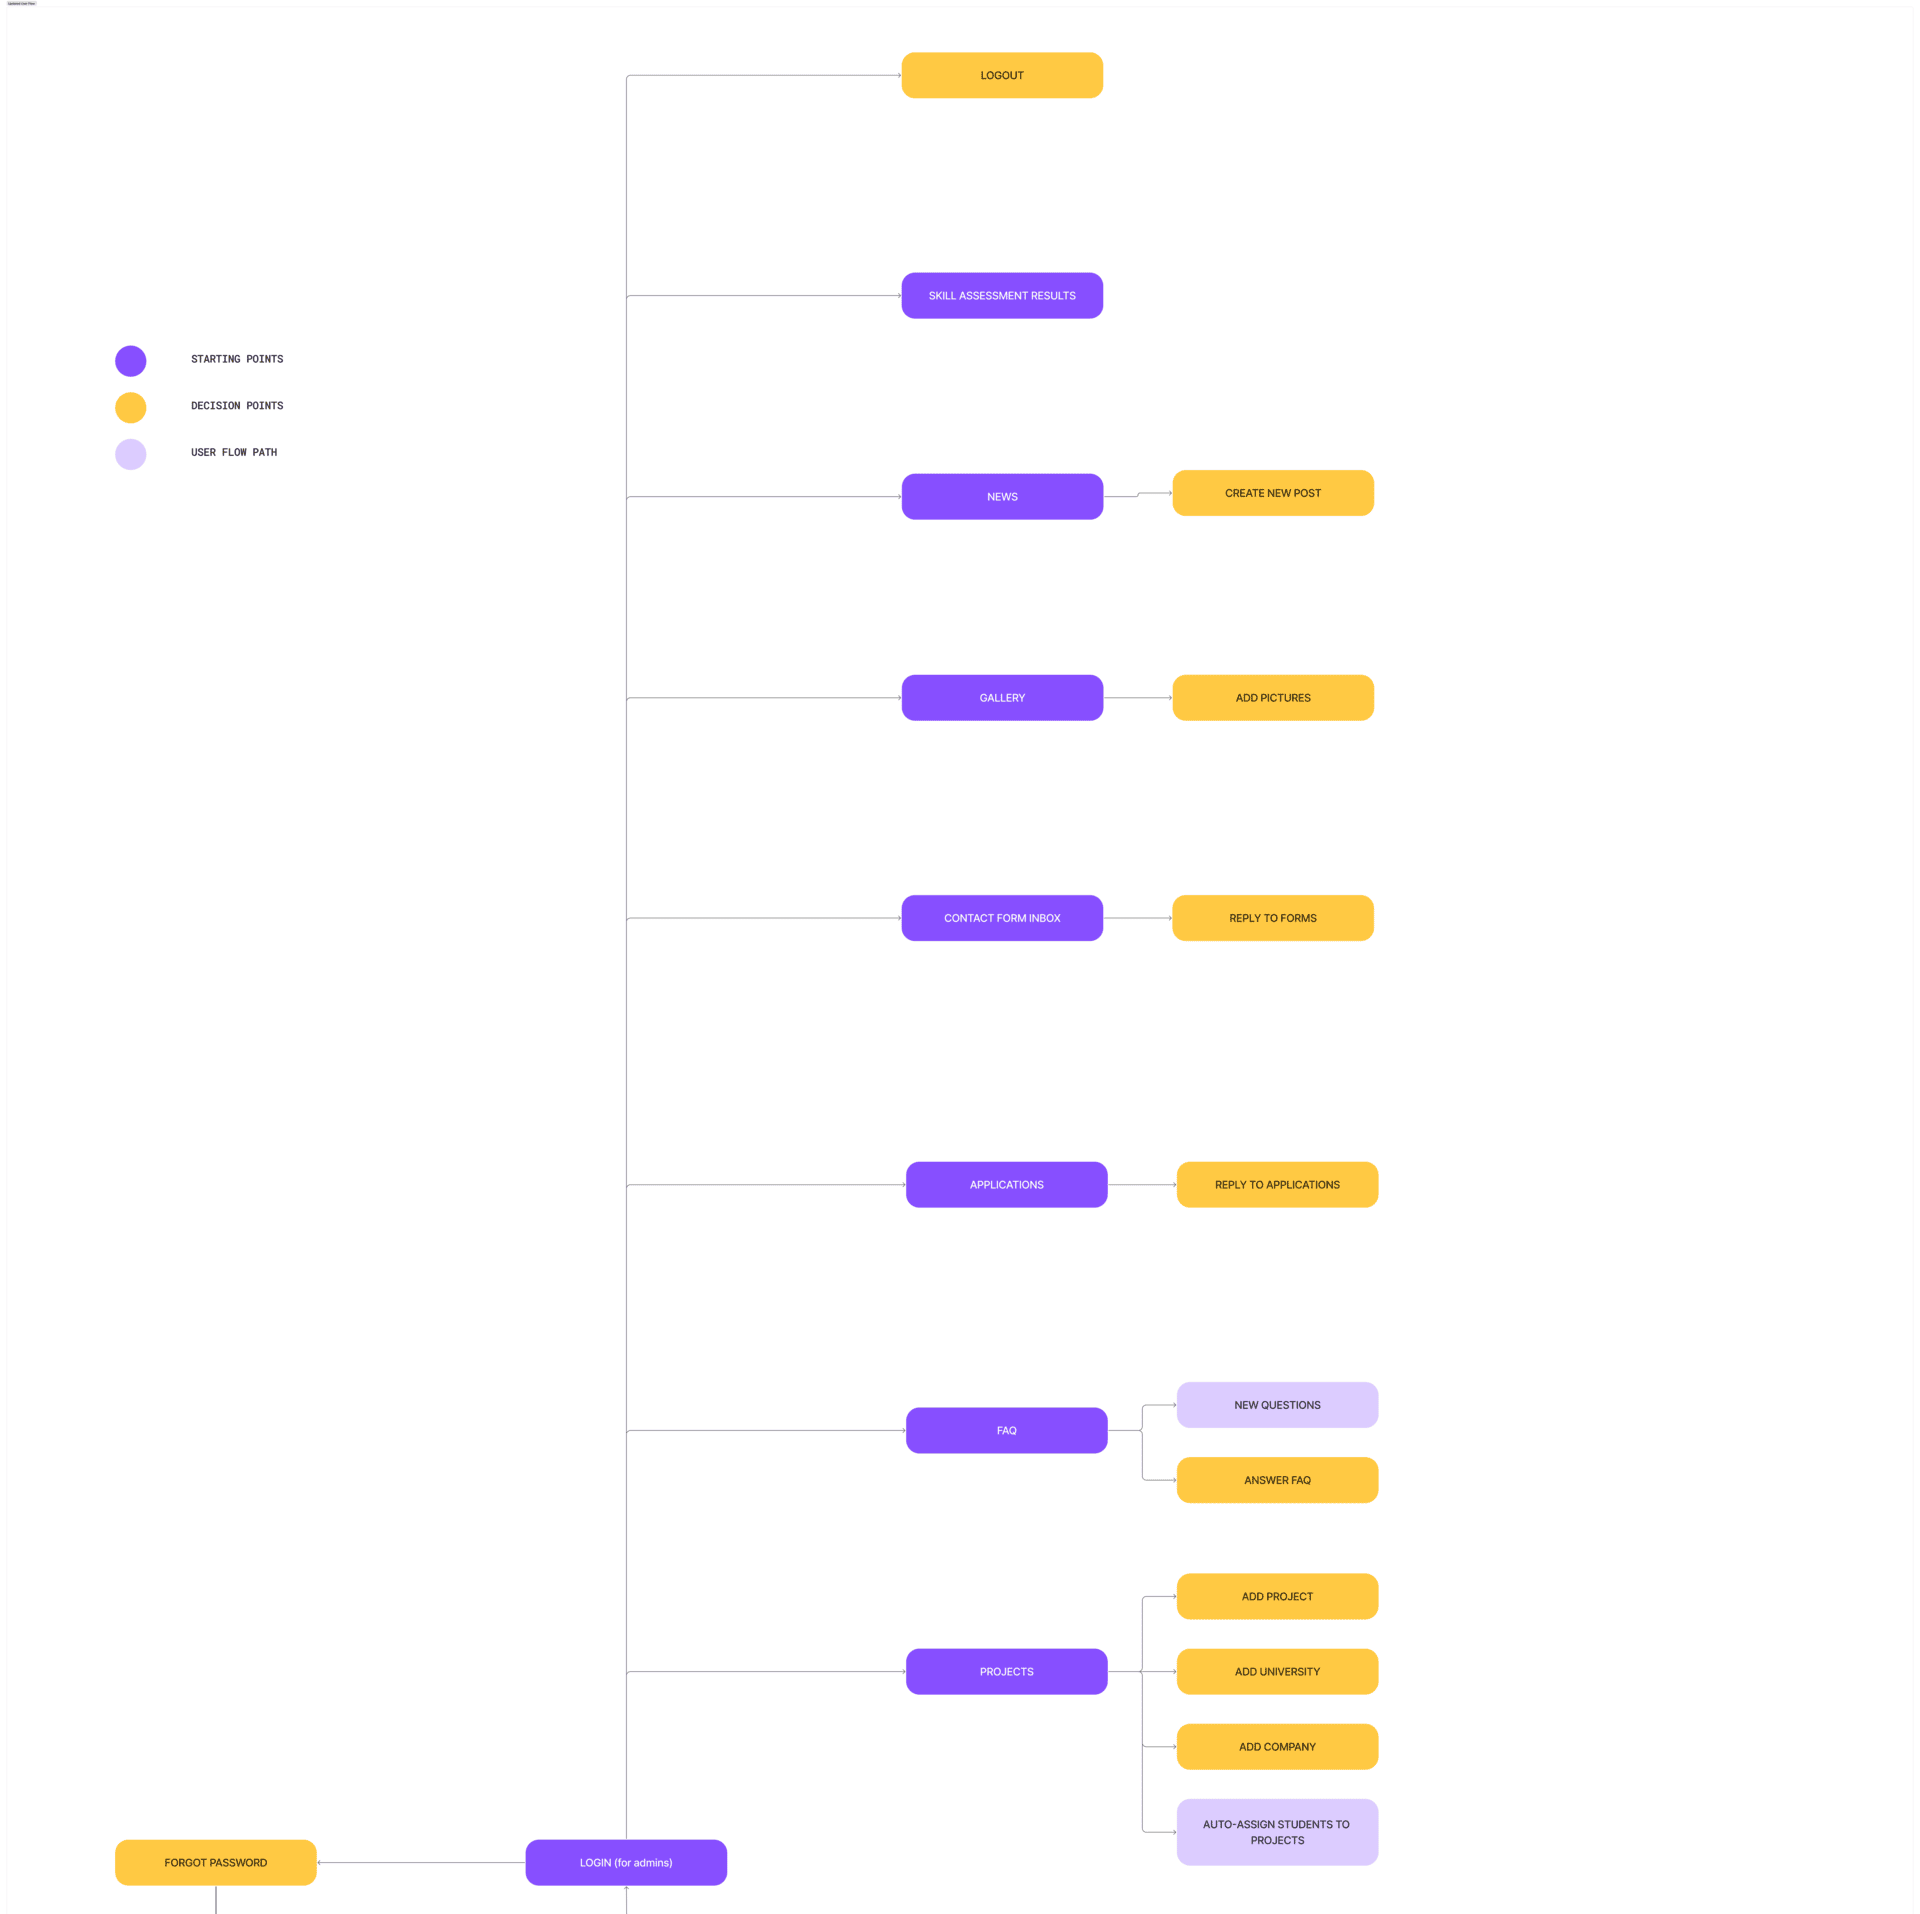
\includegraphics[width=0.85\linewidth]{appendices/a-userflowchart/BlendEd1.png}
    \caption{Diagram de User Flow da Aplicação 1}
    \label{fig:userflowchart}
\end{figure}

\begin{figure}[h!tbp]
    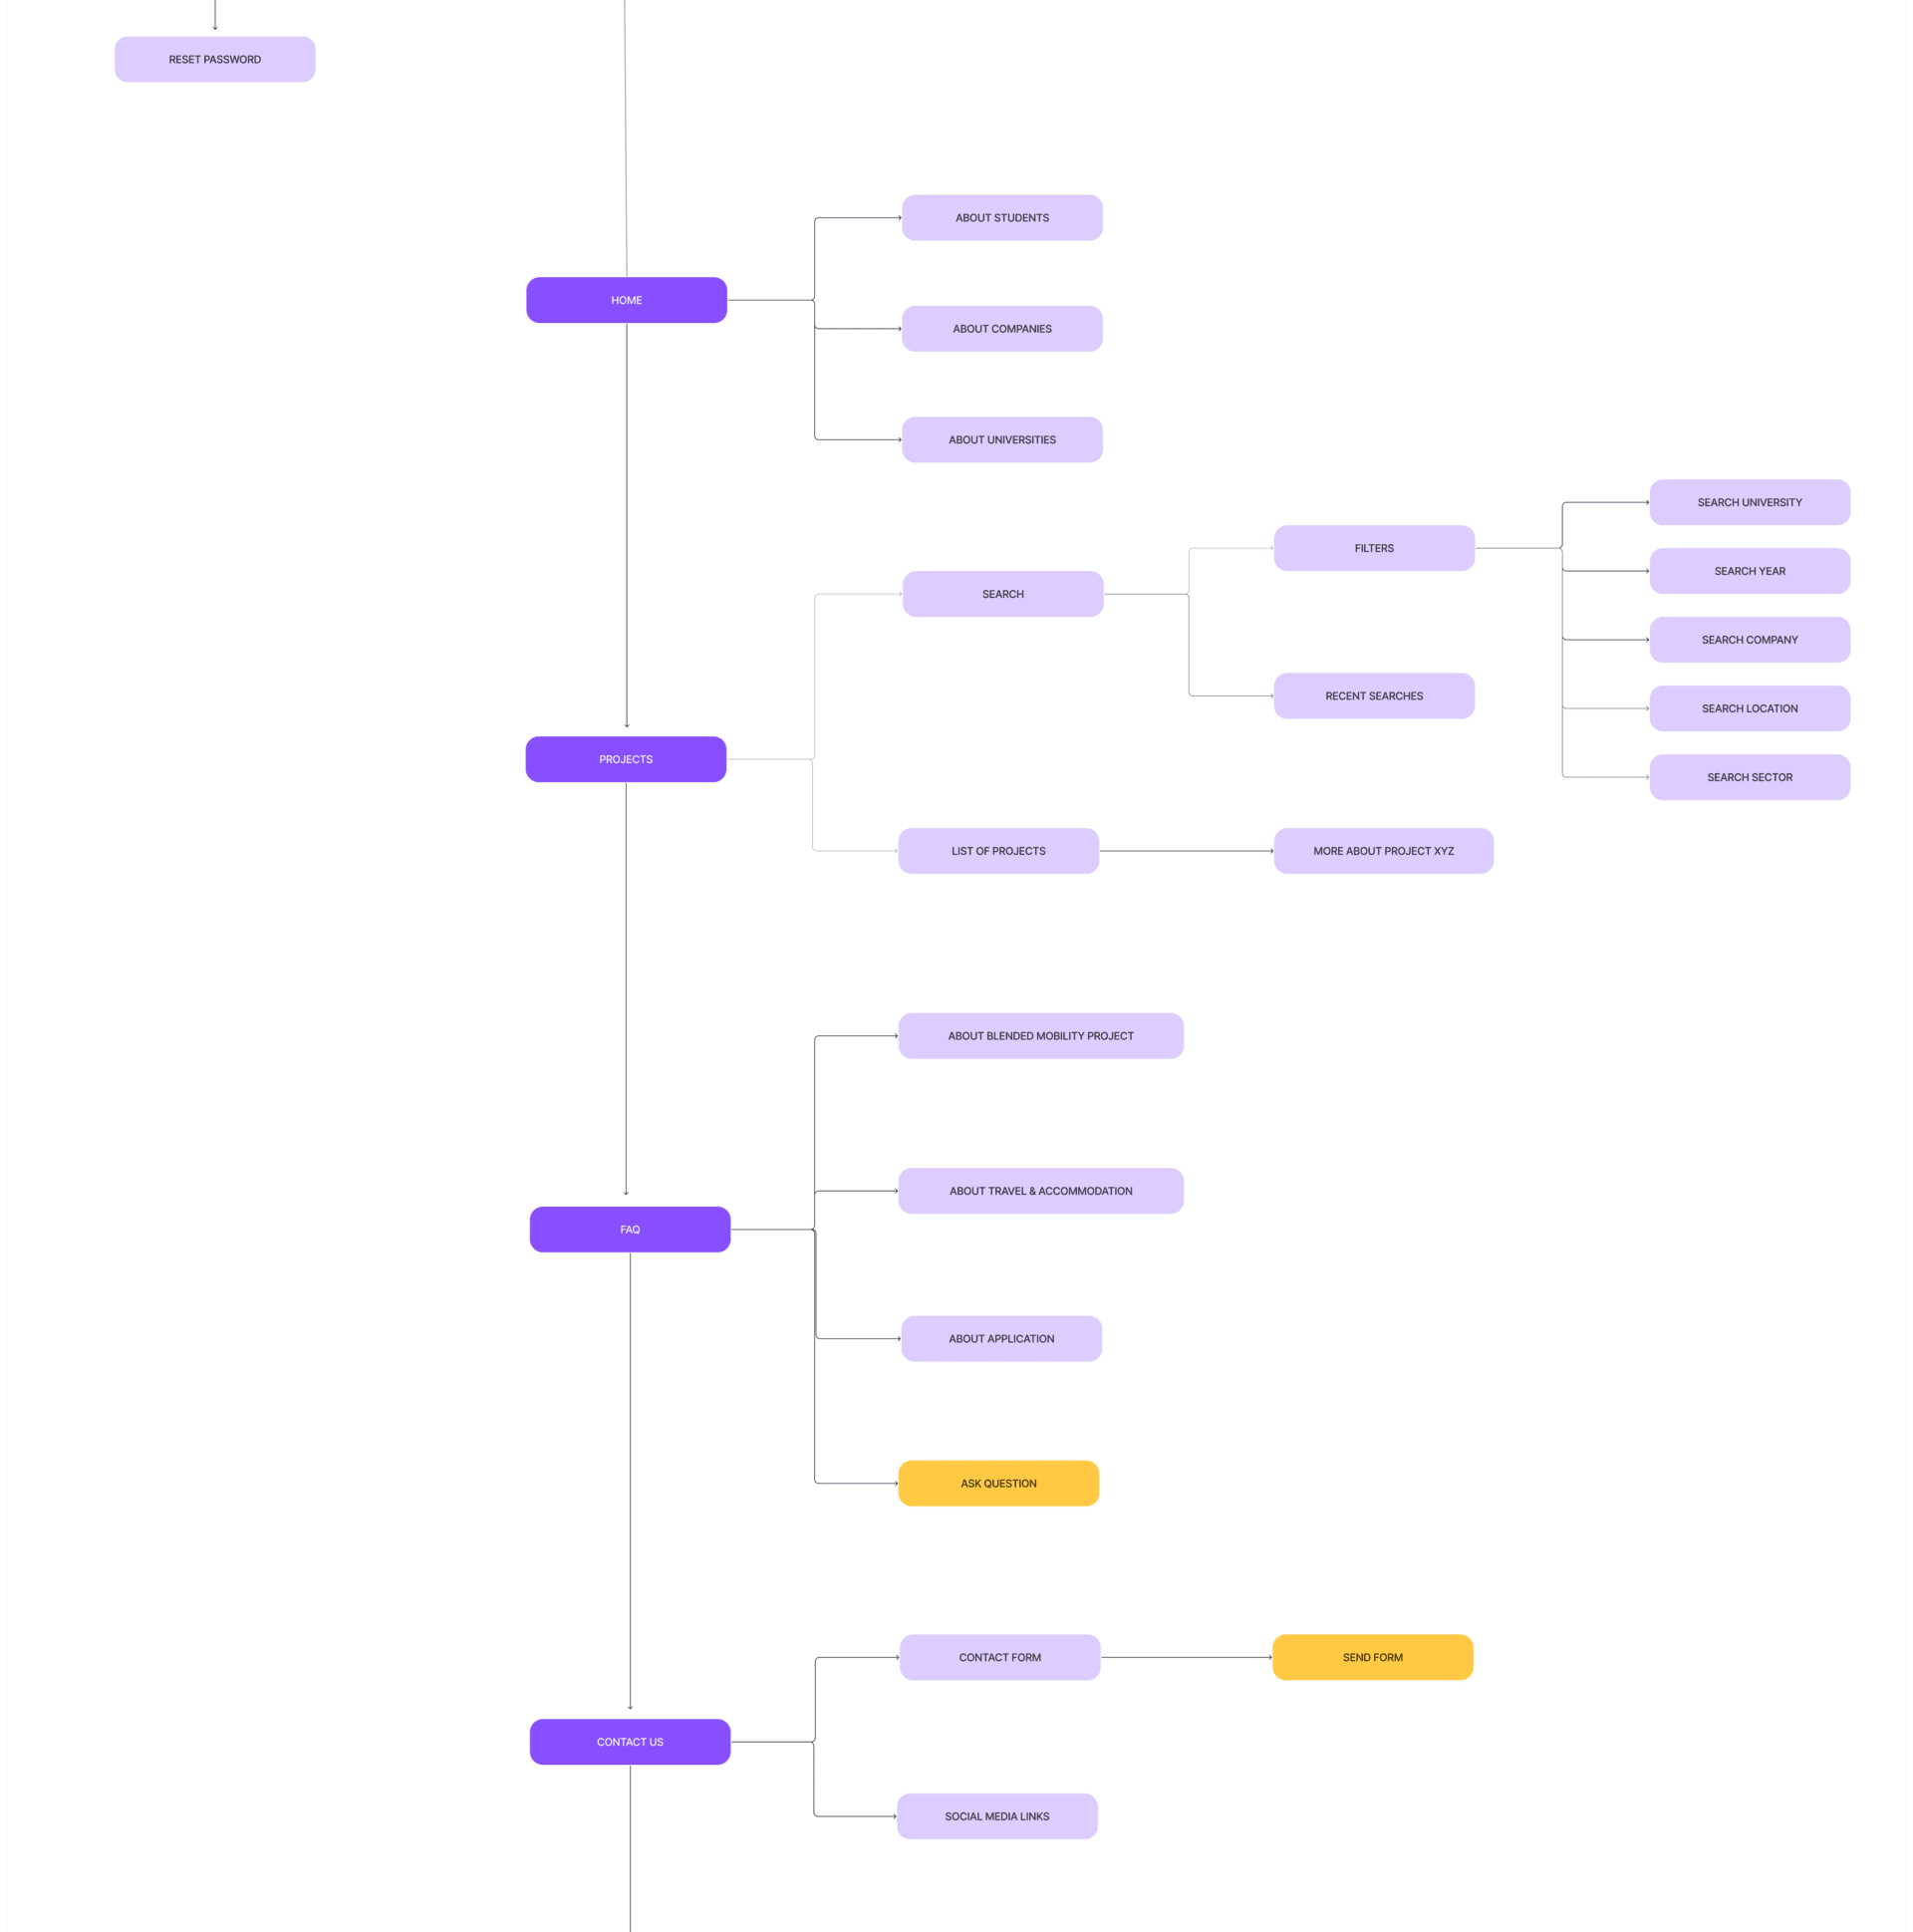
\includegraphics[width=\linewidth]{appendices/a-userflowchart/BlendEd2.png}
    \caption{Diagram de User Flow da Aplicação 2}
    \label{fig:userflowchart}
\end{figure}

\begin{figure}[h!tbp]
    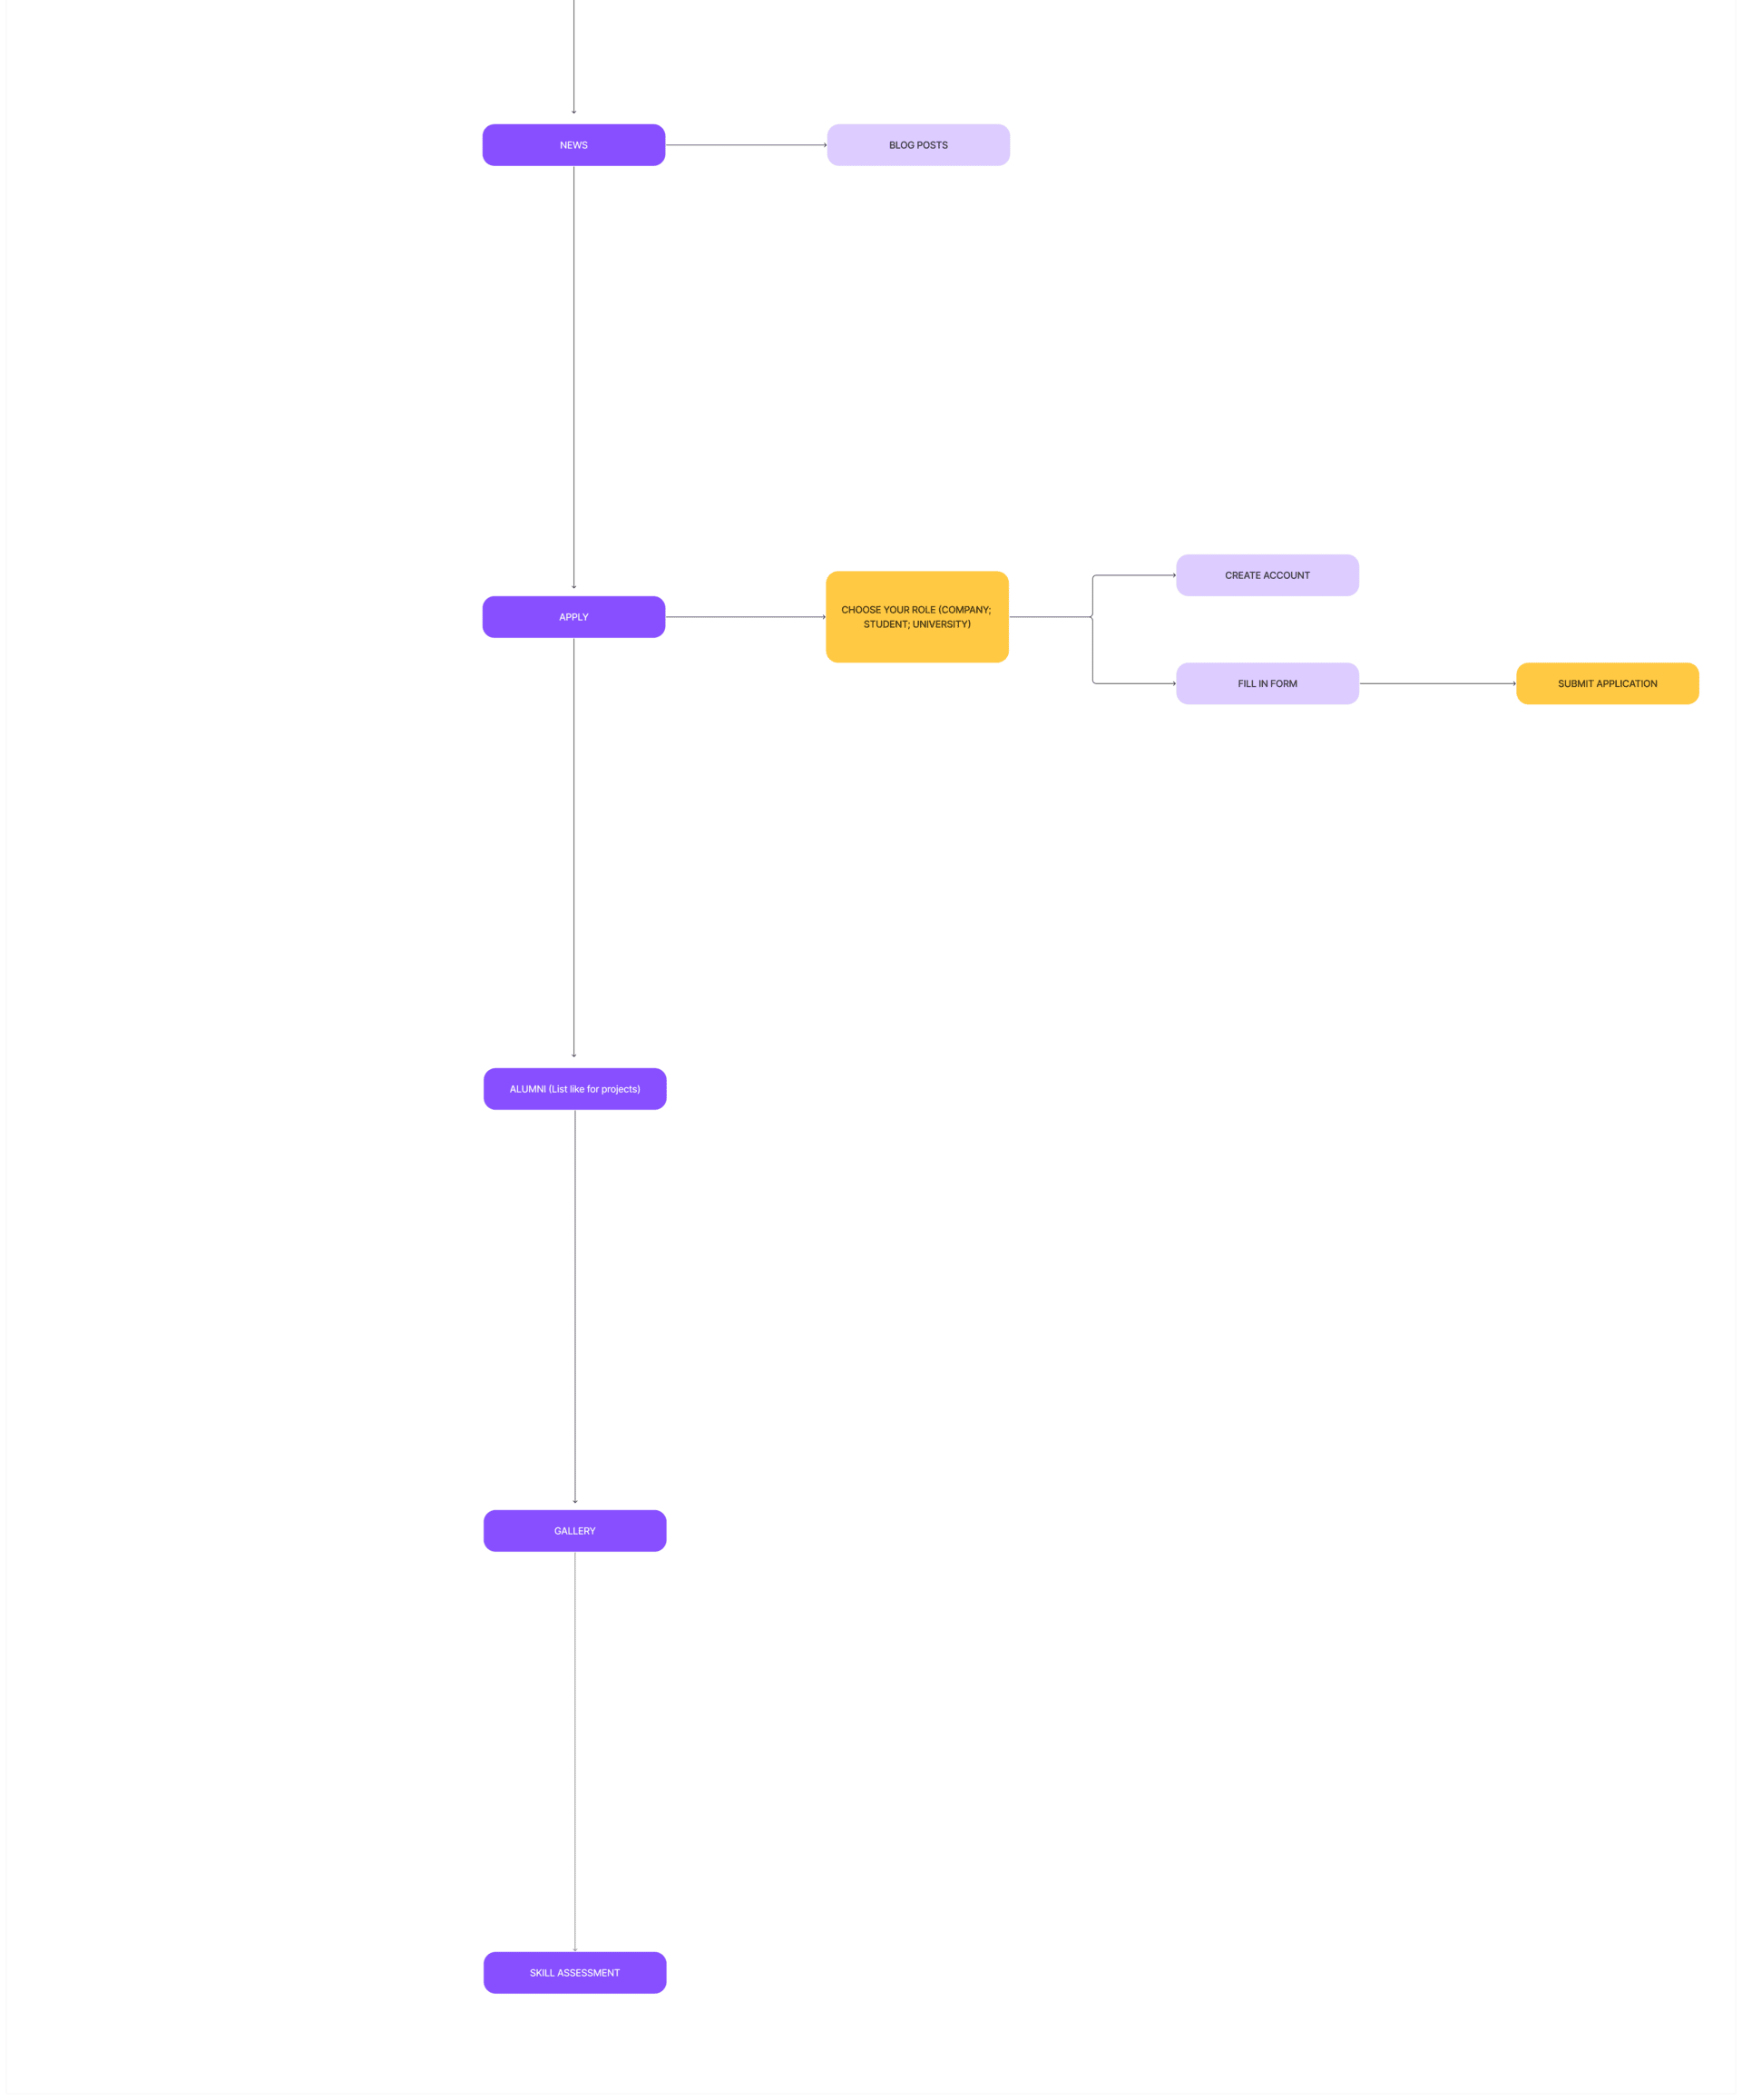
\includegraphics[width=\linewidth]{appendices/a-userflowchart/BlendEd3.png}
    \caption{Diagram de User Flow da Aplicação 3}
    \label{fig:userflowchart}
\end{figure}